%!TEX encoding = utf8
%!TeX spellcheck = en_GB
%%%%%%%%%%%%%%%%%%%%%%%%%%%%%%%%%%%%%%%%%%%%%%%%%%%%%%%%%%%%%%%%%%
\documentclass{thesis}

\section{Objectives}
  The object of this work is to model, simulate and control a three-phase-inverter by using MATLAB-Simulink. The control has to function properly under balanced steady-state conditions and under three-phase faults.

\section{Problem definition}
  Having an inverter with the following characteristics, implement and control the system in Simulink.

  \begin{figure}[H]
    \centering
    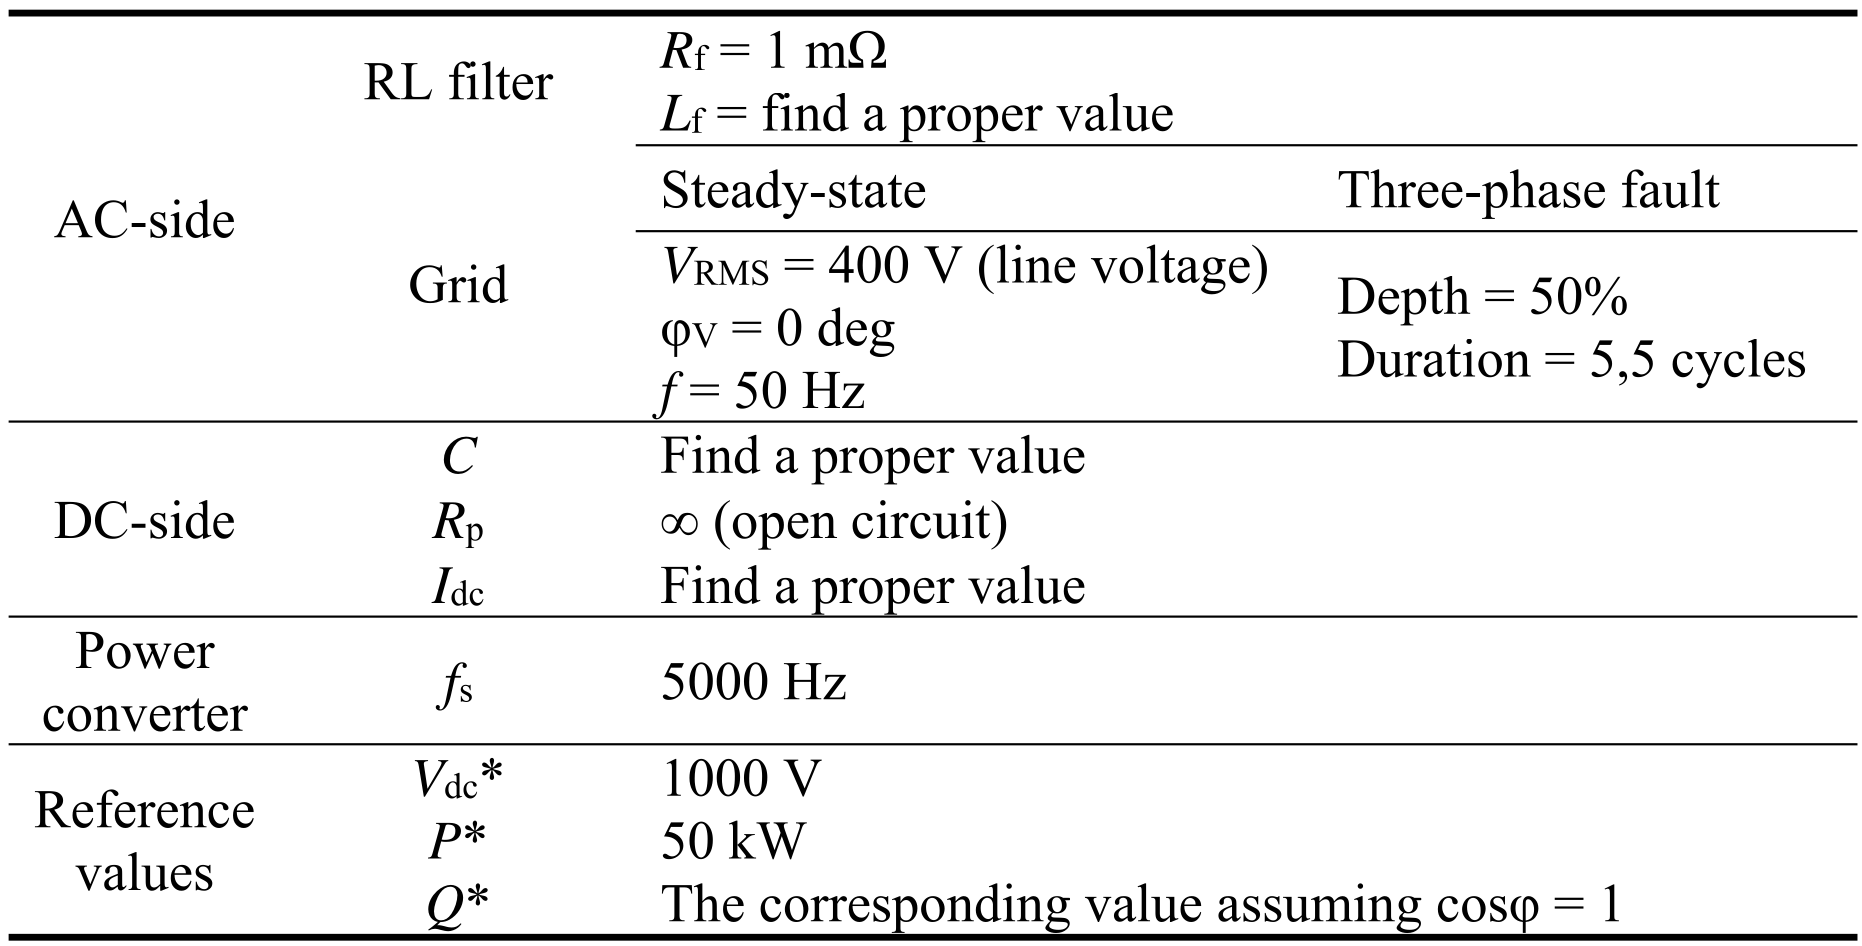
\includegraphics[width=.8\linewidth]{Images/Three-phaseInverterParameters.png}
    \caption{Inverter characteristics}
    \label{InverterData}
  \end{figure}
  \begin{figure}[H]
    \centering
    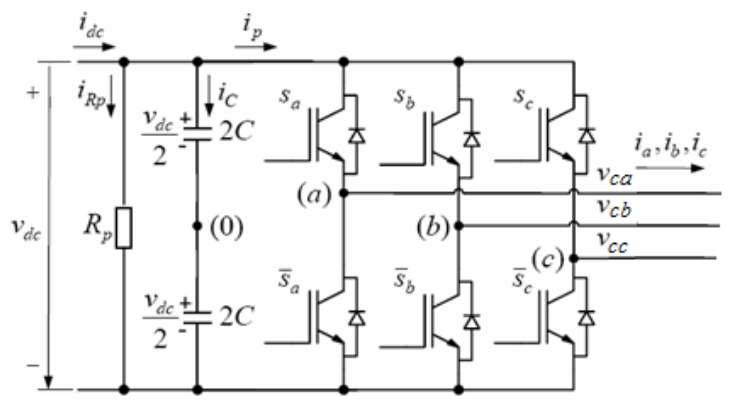
\includegraphics[width=.7\linewidth]{Images/Converter_fig.png}
    \caption{Inverter connected to the grid}
    \label{Converter_fig}
  \end{figure}

\section{Theoretical framework}
    A power inverter is a power electronic device that changes DC current into AC current by means of controlled switching an array of transistors, thus inverters are capable of outputting different voltages and frequencies with high levels of efficiency. Inverters have seen wide adoption in electric motor speed control, renewable energy generation such as wind and solar or for their use in uninterrupted power supplies.\\

  \subsection{Motor control using inverters}
      \subsubsection{Scalar control}
        Scalar control only controls the magnitude and frequency of the supply voltage that are controlled without phase control and it is suitable for application where the load is constant, otherwise vector control should be used in order to control both speed and torque.

      \subsubsection{Vector control}
        Vector control or field-oriented control (FOC), is a variable-frequency drive control method in which the stator currents of a three-phase AC electric motor are identified as two orthogonal components that can be visualized with a vector. One of the components defines the magnetic flux of the motor, the other the torque (d and q frame). The control system of the drive calculates the corresponding current component references from the flux and torque references given by the drive's speed control. Typically proportional-integral (PI) controllers are used to keep the measured current components at their reference values. The pulse-width modulation of the variable-frequency drive defines the transistor switching according to the stator voltage references that are the output of the PI current controllers.\\

        The three-phase voltages, currents and fluxes of AC-motors can be analyzed in terms of complex space vectors, for this application 3 different spaces are used. The a,b,c frame represents the three phase currents on 3 time dependent variables and is a commonplace frame of reference, however is not ideal when designing a control system, so it needs to be transformed into a two time invariant coordinate system. This transformation can be divided into two steps:
        \begin{itemize}
          \item (a, b, c) -> $(\alpha, \beta)$ (the Clarke transformation), which gives outputs of two coordinate time variant system.
          \item $(\alpha, \beta)$ -> (d, q) (the Park transformation), which gives outputs of two coordinate time invariant system.
        \end{itemize}

        \subsubsection{Vector control application step by step}
          \begin{enumerate}
            \item Stator phase currents are measured, converted to complex space vector in (a,b,c) coordinate system.
            \item Current is converted to $(\alpha, \beta)$ coordinate system. Transformed to a coordinate system rotating in rotor reference frame, rotor position is derived by integrating the speed by means of speed measurement sensor.
            \item Rotor flux linkage vector is estimated by multiplying the stator current vector with magnetizing inductance $L_m$ and low-pass filtering the result with the rotor no-load time constant $L_r/R_r$, namely, the rotor inductance to rotor resistance ratio.
            \item Current vector is converted to (d,q) coordinate system.
            \item d-axis component of the stator current vector is used to control the rotor flux linkage and the imaginary q-axis component is used to control the motor torque. While PI controllers can be used to control these currents, bang-bang type current control provides better dynamic performance.
            \item PI controllers provide (d,q) coordinate voltage components. A decoupling term is sometimes added to the controller output to improve control performance to mitigate cross coupling or big and rapid changes in speed, current and flux linkage. PI-controller also sometimes need low-pass filtering at the input or output to prevent the current ripple due to transistor switching from being amplified excessively and destabilizing the control. However, such filtering also limits the dynamic control system performance. High switching frequency (typically more than 10 kHz) is typically required to minimize filtering requirements for high-performance drives such as servo drives.
            \item Voltage components are transformed from (d,q) coordinate system to $(\alpha, \beta)$ coordinate system.
            \item Voltage components are transformed from $(\alpha, \beta)$ coordinate system to (a,b,c) coordinate system or fed in Pulse Width Modulation (PWM) modulator, or both, for signaling to the power inverter section.
          \end{enumerate}

  \subsection{Why does the previous section matter?}
    Although the objective of this work is not to control a motor a very similar technique to vector control is used to control the inverter and keep it in phase with the grid.

    \begin{figure}[H]
      \centering
      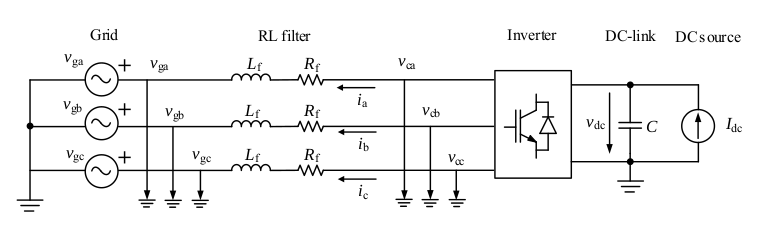
\includegraphics[width=.8\linewidth]{Images/ThreePhaseInverter_Example.png}
      \caption{Three-phase inverter connected to the grid}
      \label{ModelFig}
    \end{figure}

  \subsection{Why use an RL filter?}
    As can be observed on the previous figure there is an RL filter between the inverter and the grid. This filter is placed to eliminate the non sinusoidal components of the output wave of the inverter that result from the imperfect switching. In order to obtain a suitable value the following formula can help us:
    \begin{equation}
      L_f\approx\frac{\frac{V_{dc}/2}{\sqrt{2}}}{2*\pi*f_s*\frac{3}{2}*i_{rippleAdm}}
    \end{equation}
